\documentclass[border=10pt]{standalone}
\usepackage{tikz}
\usetikzlibrary{intersections, calc}

\begin{document}

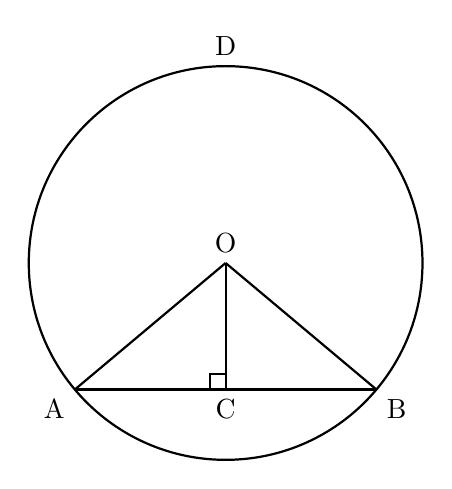
\begin{tikzpicture}[scale=1, thick]

    % 1. Define Center O and Radius
    \coordinate (O) at (0,0);
    \def\radius{2.5}

    % 2. Draw the main circle
    \draw (O) circle (\radius);

    % 3. Define point D at the top
    \coordinate (D) at (0,\radius);

    % 4. Define points A and B on the circumference
    \coordinate (A) at (220:\radius);
    \coordinate (B) at (320:\radius);

    % 5. Define point C mathematically
    % This ensures OC and AB meet perfectly at the same coordinate
    \coordinate (C) at (intersection of O--(0,-3) and A--B);

    % 6. Draw the segments
    \draw (O) -- (A); % Radius OA
    \draw (O) -- (B); % Radius OB
    \draw (A) -- (B); % Chord AB
    \draw (O) -- (C); % Perpendicular OC - now perfectly connected

    % 7. Draw the Right Angle Symbol at C
    % Using relative coordinates from the exact point C
    \draw (C) -- ++(-0.2,0) -- ++(0,0.2) -- ++(0.2,0);

    % 8. Label the points exactly as shown in the image
    \node[above] at (O) {O};
    \node[above] at (D) {D};
    \node[below left] at (A) {A};
    \node[below right] at (B) {B};
    \node[below] at (C) {C};

\end{tikzpicture}

\end{document}
